\section{User manual}

\subsection{Functional requirements}
\begin{itemize}
\item Requires the user to have a android device with Android OS v2.2 or newer.
\item Requires Internet to enable online play.
\end{itemize}

\subsection{Running the application}
The application is avalible at URL. \\
The Eclipse-project is avalible at ANOTHER URL.

\subsubsection{Emulator}
To run the application in the emulator, the user needs to open the project in Eclipse.
File -> Open project -> Existing source code -> path to downloaded project.


\subsubsection{On Android device}
\paragraph*{Method 1}
To run the application on the Android device, the user needs to open the project in Eclipse.
File -> Open project -> Existing source code -> path to downloaded project.
Then connect the Android device with an USB cable to the PC, and run the project.

\paragraph*{Method 2}
Download the apk file form URL, transfer to the android device with an USB cable and explore and install the application on the device.

\subsection{Game rules}
The game is implemented with the same set of rules as the classic board game \emph{Nine Men's Morris} \cite{morris}. The goal of the game is to either block any opponent moves, or to reduce your opponent's piece number to less than three. If you get three pieces in a row, you enter a morris state, and are allowed to remove one of your opponent's pieces. Pieces that are in a morris state, i.e. forms three in a row either horizontally or vertically, are not removable.

\subsection{Creating Skiller account}
The first thing that meets the user after starting the application for the first time, is a Skiller dialogue asking the user to create a Skiller account. This account will later be used for playing the game online.

\subsection{How to play}
\label{section:playing}

\subsubsection{Choosing game mode}
A user can choose between online mode or hotseat mode. Clicking "Crate Game" or "Join Game" will start a game in online mode. Clicking "Hotseat" will start a game in hotseat mode.
\label{section:game_mode}
\begin{figure}[H]
	\centering
	\mbox{
	\subfigure[Available game modes]{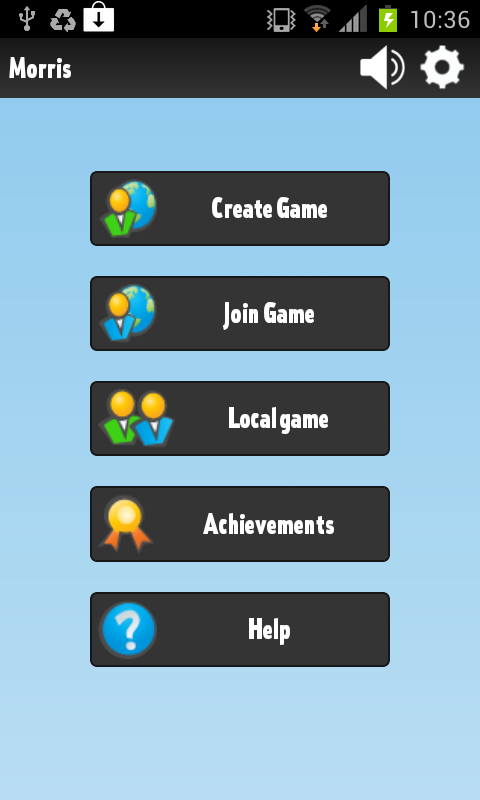
\includegraphics[width=2.1in]{Images/menuPage.png}}
	\subfigure[Achievements]{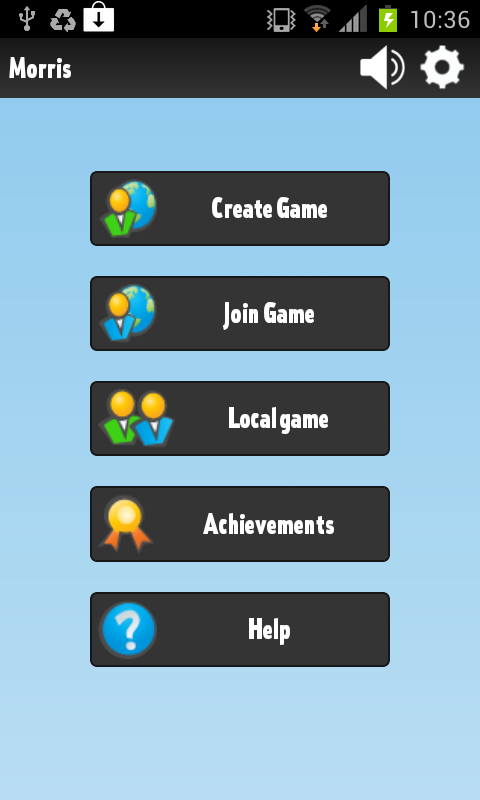
\includegraphics[width=2.1in]{Images/menuPage.png}}
	\subfigure[Help explaining the games rules]{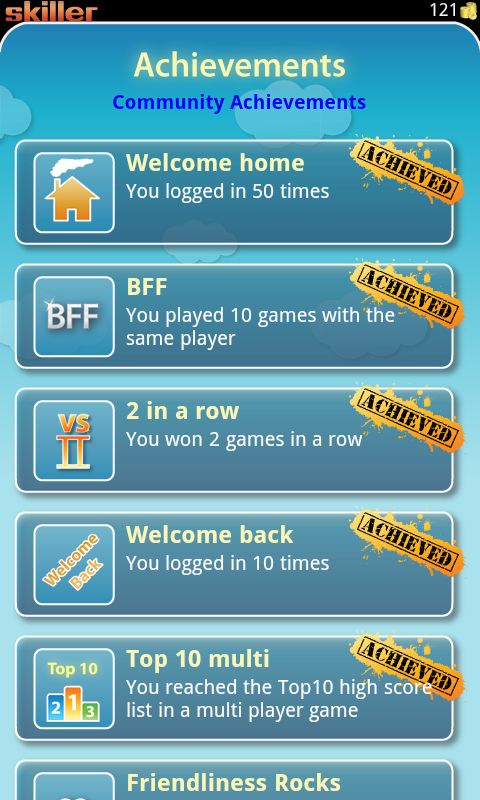
\includegraphics[width=2.1in]{Images/achievements.png}}
	}	
\end{figure}

\subsubsection{Placing, selecting, moving, and removing pieces}
When it is your turn to move, either the board or your pieces will be highlighted. In addition, the name of the current player will be blinking as the game progresses. \\
\begin{figure}[H]
	\centering
	\mbox{\subfigure[Green indicator shows where you can place a piece]{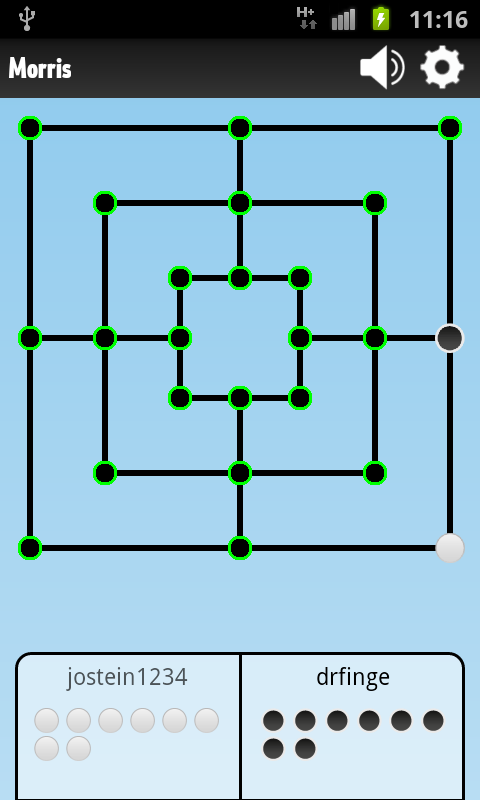
\includegraphics[width=2.1in]{Images/placementState.png}} \qquad
	\subfigure[Highlights selectable pieces]{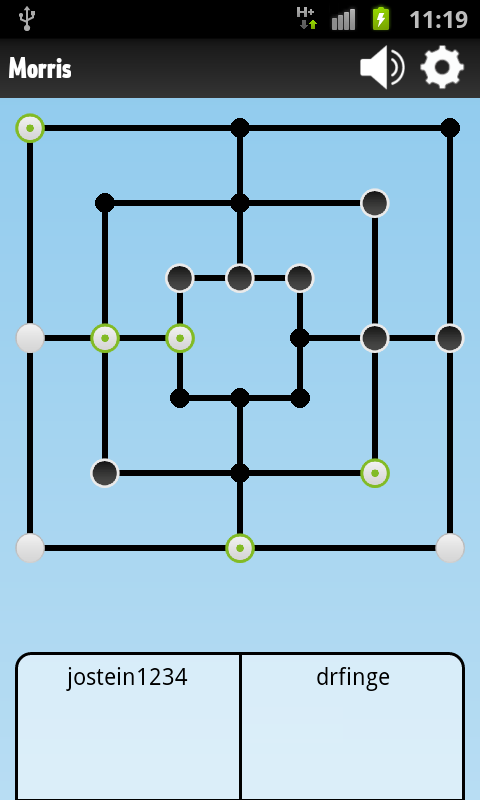
\includegraphics[width=2.1in]{Images/selectState.png}}}
	\mbox{\subfigure[Highlight selected piece, green indicator on possible moves]{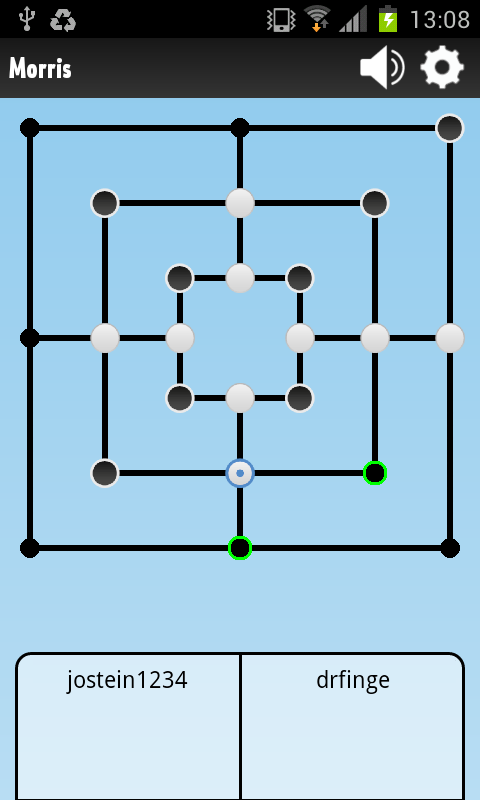
\includegraphics[width=2.1in]{Images/selectedPiece.png}} \qquad
	\subfigure[Highlights removable pieces with a red cross]{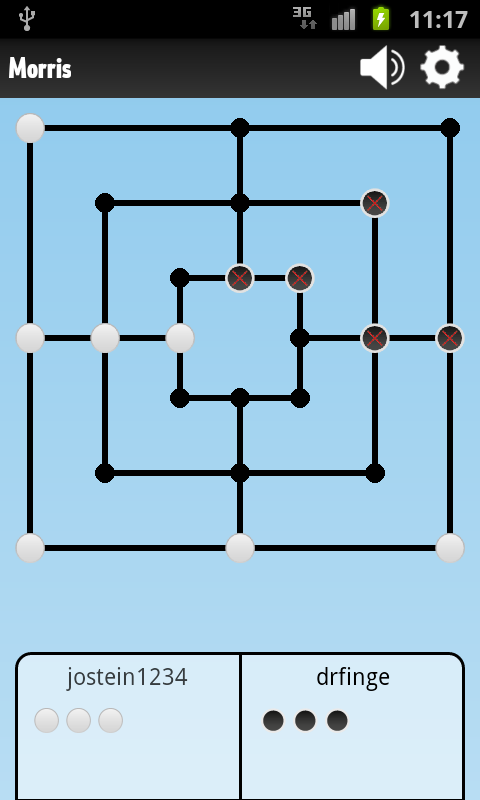
\includegraphics[width=2.1in]{Images/removalState.png}}}
\end{figure}

\subsubsection{Hotseat mode}

If you start a local game as described in section \ref{section:game_mode}, you can control both players from the same device.

\subsubsection{Online mode}

If you start an online game as described in section \ref{section:game_mode}, you are taken to the board screen, and need to wait for another player to join your game. The guest, i.e. the one who joins the game, will get the initial move. Your own pieces will always be white.






